```tex
\documentclass[conference]{IEEEtran}
\IEEEoverridecommandlockouts
\overrideIEEEmargins
\usepackage{amsmath}
\usepackage{amssymb}
\usepackage{cite}
\usepackage{graphicx}
\usepackage{booktabs}
\usepackage{tikz}
\usepackage{pgfplots}
\usepackage{algorithm}
\usepackage{algpseudocode}
\usepackage{array}
\usepackage{multirow}
\usepackage{siunitx}
\usepackage{flushend}
\pgfplotsset{compat=1.18}

\title{Optimized Values vs Base Values in Dataset-Driven Multi-Runway Flight Scheduling Using AERIS-OPT}

\author{%
\IEEEauthorblockN{Kommi Druthendra, G. Sai Santhosh, K. Dhanush, K. Jushal Reddy, Prdeepa M}
\IEEEauthorblockA{Integrated M.Tech Software Engineering, VIT Vellore}
}

\begin{document}
\maketitle

\begin{abstract}
At high-traffic airports, runway planning has to satisfy safety limits, economic pressure, and controller usability all together. With multiple runways, assignment decisions, wake-separation constraints, and release times influence one another continuously, so improving only one metric often worsens another. In this study, AERIS-OPT is applied as a staged optimization process on \texttt{flight\_data.csv} to maintain that balance in a transparent way.

The pipeline brings together candidate diversification, strict multi-metric ranking, local schedule correction, displacement smoothing, and baseline verification inside one repeatable procedure. Every method in the comparison is tested on the same input and with the same metric definitions. Along with endpoint values, we report diagnostic evidence such as demand shape, runway-balance behavior, convergence pattern, and relative-gain plots so the final choice can be followed clearly.

For the evaluated case, AERIS-OPT reaches a delay cost of 37472.9 CNY, displacement of 1.8333, and a 900-second scheduling window while satisfying configured targets. Compared with the base-reference setting reported in earlier runway research \cite{ref19}, the obtained schedule gives lower economic cost and steadier sequencing behavior. Overall, this work delivers a reproducible, operations-oriented framework for multi-runway scheduling.
\end{abstract}

\begin{IEEEkeywords}
Flight Scheduling, Runway Optimization, AERIS-OPT, Metaheuristics, Delay Minimization
\end{IEEEkeywords}

\section{Introduction}
Runway sequencing is among the most delicate tasks in airport operations. Even a small reorder near the queue front can propagate into wake-separation conflicts, runway-occupancy shifts, and extra intervention load later on. This effect becomes even more visible when two runways are active, since assignment and sequencing keep interacting across the full planning horizon.

Conventional baselines are still useful as reference points, yet dense demand exposes their limits. FCFS is straightforward to explain and deploy, but it does not directly optimize weighted delay cost. Genetic approaches enlarge search coverage, though stability can vary with parameter settings \cite{ref5,ref7}. MILP models provide strong formal constraint control, but computational effort can rise quickly as coupling increases \cite{ref9,ref11}. Earlier studies, including the improved-GA dynamical time-window approach by Zhou and Jiang \cite{ref19}, established important foundations; still, reproducible multi-metric balancing remains difficult in real use.

Another point worth noting is that runway schedules are judged by groups with different priorities. Airlines focus on delay-related cost, controllers need manageable and safe sequence flow, and airport operations teams monitor throughput and timing compactness. So, a plan that looks best from one perspective may still be inconvenient to execute in tower conditions.

For that reason, AERIS-OPT is organized as a staged runway-scheduling workflow centered on practical balance. Candidate diversity, threshold-aware filtering, local refinement, and displacement regulation are combined before final benchmark comparison. The goal here is not to win one metric in isolation; it is to output a schedule that can be used in realistic controller workflow.

All experiments are produced from \texttt{flight\_data.csv} using fixed settings and consistent metric definitions. In addition to final scores, diagnostic views are included so readers can trace why one schedule is preferred over others.

From a method standpoint, the workflow formalizes multi-objective scheduling through staged optimization and strict score governance. From a practical standpoint, the reported tables and diagnostics can be audited directly by students and practitioners, helping bridge the gap between model output and operational interpretation.

The remainder of the paper is structured as follows. Section II reviews related work. Section III introduces the formulation. Sections IV and V describe dataset and methodology. Section VI details the experimental protocol. Section VII reports findings. Section VIII discusses implications and validity limits. Sections IX and X provide conclusion and future directions.

The major contributions are summarized below.
\begin{itemize}
    \item A complete multi-runway optimization pipeline tied directly to \texttt{flight\_data.csv}.
    \item A strict scoring mechanism that jointly enforces delay-cost, displacement, and window targets.
    \item A local refinement stage that improves schedule feasibility without breaking objective gains.
    \item A reproducible comparison framework against FCFS, GA, and MILP baselines.
\end{itemize}

\section{Literature Review}
This section organizes prior runway-scheduling studies into four families and relates each family to the AERIS-OPT design choices.

\subsection{Traditional Scheduling Methods}
Deterministic runway research forms the formal core of sequencing theory. Atkin \textit{et al.} modeled airport ground-movement planning with operations-research structure and demonstrated that disciplined coordination can stabilize routine traffic \cite{ref1}. In many cases, however, adaptability weakens when queue states change abruptly.

Dorndorf \textit{et al.} examined airport scheduling complexity and clarified why conflict handling scales combinatorially with interacting resources \cite{ref2}. Their analysis is theoretically strong, but complexity characterization alone does not directly produce tactical control rules.

Beasley \textit{et al.} proposed a separation-constrained landing formulation that remains influential for safety-driven sequencing \cite{ref3}. The key advantage is explicit feasibility management, while scalability drops when richer multi-runway interactions are introduced.

Bianco \textit{et al.} embedded congestion-aware constraints into deterministic scheduling formulations \cite{ref4}. This improves structured control, though fixed assumptions can limit responsiveness during irregular peaks.

\subsection{Genetic Algorithm Methods}
Metaheuristic work broadened exploration beyond rigid deterministic orderings. Pinol and Beasley showed that population-based sequence search can escape weak local minima in constrained landing settings \cite{ref5}. Search diversity improves, but output quality depends strongly on parameter tuning and termination criteria.

Sabar and Kendall introduced population-based hyper-heuristics that adapt operator selection during search \cite{ref6}. This raises exploration flexibility, although runtime behavior can become volatile under tightly constrained operational windows.

Zhou \textit{et al.} reported GA-based collaborative optimization for multi-runway control \cite{ref7}. Their framework improves over FCFS in global search quality, yet performance remains sensitive to crossover and mutation design.

Lieder and Stolletz incorporated uncertainty-aware adaptation for sequencing under variable arrivals \cite{ref8}. Robustness improves, but calibration effort increases when uncertainty patterns differ between airports.

\subsection{MILP-Based Methods}
MILP remains one of the clearest ways to encode strict runway constraints. Balakrishnan and Chandran formulated constrained position shifting to limit excessive reordering while preserving explicit feasibility \cite{ref9}. Reliability is high, but solving effort rises with additional interaction detail.

Bennell \textit{et al.} surveyed exact and approximate runway optimization methods and reinforced MILP as a strong formal mechanism for feasibility control \cite{ref10}. The same survey also emphasizes a recurring issue: exact models become costly on larger dense instances.

Hu and Chen unified runway assignment and sequencing in a mixed-integer model \cite{ref11}. Internal consistency is improved, though model size and runtime expand rapidly for wider tactical horizons.

Schuster and Ochieng studied resilient runway optimization under disturbances \cite{ref12}. They improve reliability in disrupted contexts, while tractability remains the main practical bottleneck.

\subsection{Hybrid and Data-Driven Methods}
Hybrid research combines structured optimization with adaptive ranking or learning signals. Ikli \textit{et al.} found that hybrid families often provide stronger trade-offs than single-technique pipelines \cite{ref13}. The downside is added implementation complexity and higher tuning demand.

Kim \textit{et al.} presented learning-assisted runway sequence control with improved adaptation \cite{ref14}. Their findings also suggest that explicit post-processing is still needed to preserve strict feasibility.

Wang \textit{et al.} used graph-based decision support to represent movement dependencies explicitly \cite{ref15}. This helps with relational conflict handling, though deployment overhead increases when graph updates are frequent.

Li \textit{et al.} reported competitive constrained performance with hybrid metaheuristics \cite{ref16}. A remaining concern is parameter transferability across airports with different traffic mixes.

The base paper by Zhou and Jiang \cite{ref19} is especially relevant here because it demonstrated improved-GA scheduling with a dynamical time-window strategy and reported clear reductions in delay and workload. For the present study, a practical limitation is that broader reproducibility and diagnostic transparency were less emphasized.

\subsection{Research Gap}
Two gaps are still evident. First, many methods are strong either in economic optimization or strict feasibility, but fewer support reliable joint control of delay cost, displacement, and compact scheduling window in one reproducible process. Second, several studies report final metrics without detailed stage-level diagnostics. AERIS-OPT addresses both gaps through strict multi-factor scoring and explicit convergence/sensitivity reporting.

There is also an explainability gap in student-level implementation settings. Strong endpoint scores are often shown without enough visibility into why one candidate is selected when constraints are close. The current workflow addresses this by pairing strict ranking logic with readable diagnostics, so decisions can be audited beyond a single score table.

\begin{table}[t]
\centering
\caption{Summary taxonomy of runway scheduling method families}
\small
\begin{tabular}{p{1.8cm} p{2.15cm} p{1.6cm} p{1.55cm}}
\toprule
Family & Typical strength & Key risk & Main references \\
\midrule
Rule-based (FCFS) & Fast and transparent deployment & Poor global optimality under congestion & \cite{ref1,ref4} \\
GA and metaheuristics & Strong search diversity & Parameter sensitivity and runtime variance & \cite{ref5,ref6,ref7} \\
MILP & Precise constraint control & Scalability limits for dense interactions & \cite{ref9,ref10,ref11} \\
Hybrid data-driven & Better metric balance and robustness & Additional tuning and implementation complexity & \cite{ref13,ref14,ref15,ref16} \\
\bottomrule
\end{tabular}
\label{tab:litsummary}
\end{table}

Table~\ref{tab:litsummary} motivates selecting a hybrid staged optimizer that preserves deterministic explainability while benefiting from multi-seed exploration.

\section{Problem Formulation}
Let $\mathcal{F}=\{1,2,\ldots,N\}$ denote flights and $\mathcal{R}=\{1,2,\ldots,R\}$ denote runways.

\subsection{Decision Variables}
\begin{itemize}
    \item $x_{ir} \in \{0,1\}$: 1 if flight $i$ is assigned to runway $r$.
    \item $t_i \in \mathbb{R}_{\ge 0}$: scheduled time for flight $i$.
    \item $y_{ijr} \in \{0,1\}$: 1 if flight $i$ is sequenced before flight $j$ on runway $r$.
\end{itemize}

\subsection{Objective}
The primary objective minimizes weighted delay cost:
\begin{equation}
\min Z = \sum_{i\in\mathcal{F}} c_i\,\max(0, t_i-\eta_i)
\label{eq:objective}
\end{equation}
where $\eta_i$ is the readiness time and $c_i$ is unit delay cost.

To support multi-objective behavior in one executable pipeline, we use a strict score during candidate ranking:
\begin{equation}
S(\pi)=\alpha\,\widehat{C}(\pi)+\beta\,\widehat{D}(\pi)+\gamma\,\widehat{W}(\pi)+\lambda\,\Phi(\pi)
\label{eq:strictscore}
\end{equation}
where $\widehat{C},\widehat{D},\widehat{W}$ are normalized delay, displacement, and window terms, and $\Phi(\pi)$ is a penalty that activates when threshold constraints are violated. This formulation keeps selection behavior interpretable and prevents candidates with severe trade-off imbalance from dominating by cost alone.

\subsection{Constraints}
\textbf{Runway assignment:}
\begin{equation}
\sum_{r\in\mathcal{R}} x_{ir}=1,\quad \forall i\in\mathcal{F}
\label{eq:assign}
\end{equation}

\textbf{Runway separation:}
\begin{equation}
t_j-t_i \ge s_{ij}-M(1-y_{ijr})-M(2-x_{ir}-x_{jr})
\label{eq:sep}
\end{equation}
for all $i\neq j$ and each runway $r$.

\textbf{Order consistency:}
\begin{equation}
y_{ijr}+y_{jir}=1,\quad \forall i\neq j,\forall r
\label{eq:order}
\end{equation}

\textbf{Time-window feasibility:}
\begin{equation}
t_i \ge \eta_i,\quad \forall i\in\mathcal{F}
\label{eq:window}
\end{equation}

\textbf{Displacement control:}
\begin{equation}
\frac{1}{N}\sum_{i\in\mathcal{F}}\left|\pi_i-\pi_i^{\text{ref}}\right| \le D_{\max}
\label{eq:disp}
\end{equation}
where $\pi_i$ is final position, $\pi_i^{\text{ref}}$ is reference order, and $D_{\max}$ is the acceptable displacement limit.

\subsection{Operational Interpretation}
Equation~\eqref{eq:objective} captures economic delay pressure, whereas Equations~\eqref{eq:assign}--\eqref{eq:window} enforce sequencing that is safe and executable. Equation~\eqref{eq:disp} limits excessive order drift so controllers can still reason about planned movement without abrupt tactical reversals. In practical operation, the optimizer therefore must produce schedules that are not only feasible but also cheaper and easier to execute.

\subsection{Complexity Perspective}
If $K$ candidates are evaluated and each candidate performs schedule refinement over $N$ flights, dominant computational effort is approximately $\mathcal{O}(K\,N^2)$ because of repeated pairwise separation checks and local reordering operations. For tactical runway planning, this cost is generally manageable since optimization budgets are bounded and candidate pools can be parallelized. In effect, the multi-stage design exchanges modest extra computation for clearer improvements in schedule quality and interpretability.

\section{Dataset Description}
All analysis is based solely on \texttt{flight\_data.csv}, which provides the event and evaluation context used in this study. Each row includes operational fields such as \textit{Category}, \textit{Airline}, \textit{Type}, \textit{DelayCost}, \textit{Time}, and \textit{Runway}. Together, these attributes describe role, aircraft class, temporal position, and economic sensitivity for each movement.

Column usage is defined as follows. \textit{Category} marks operational direction (arrival or departure), affecting queue interaction patterns. \textit{Airline} and flight identifiers are kept for traceability. \textit{Type} (L/M/H) maps movements to wake-separation behavior. \textit{EstimatedTime} provides the baseline temporal anchor. \textit{UnitDelayCost} quantifies per-unit economic impact of delay. \textit{Runway} stores assignment information for conflict and utilization analysis.

Arrivals and departures are solved in a unified schedule because they compete for the same runway resources and safety margins. Aircraft classes L, M, and H are mapped into wake-dependent feasibility constraints, keeping safety logic explicit through optimization.

Arrival and departure events do not contribute equally to schedule pressure. Arrival delays can propagate quickly to gate and turnaround processes, while departure delays may affect downstream slot compliance and network punctuality. Modeling both categories together allows shared-runway competition to be handled while maintaining class-dependent spacing safety.

Delay cost is computed from positive temporal deviation weighted by per-flight delay coefficients. This dataset is suitable for runway optimization because timing, class, and cost appear in one consistent structure, enabling direct feasibility checks and objective evaluation without synthetic data construction.

Formally, if $\Delta_i=\max(0,t_i-\eta_i)$ is the positive delay for flight $i$, then the flight-level delay-cost contribution is $c_i\Delta_i$, where $c_i$ is taken from the per-flight unit delay cost field. As a result, economically sensitive flights receive proportionally stronger priority during optimization.

Table~\ref{tab:datasetpreview} provides a raw-data snapshot. Fig.~\ref{fig:datasetprofile} summarizes category and type distribution used by the optimizer.

\begin{table*}[t]
\centering
\caption{Dataset preview from \texttt{flight\_data.csv}}
\scriptsize
\begin{tabular}{l l c l c c c c}
\toprule
Category & Airline & Number & FlightNumber & Type & UnitDelayCost & EstimatedTime & Runway \\
\midrule
Departure & CES & 1 & MU5990 & M & 2.0 & 00:00:00 & 0 \\
Departure & CCA & 8 & CA4307 & H & 4.0 & 00:04:00 & 0 \\
Departure & CSC & 12 & 3U8869 & H & 4.1 & 00:08:00 & 1 \\
Arrival & CSC & 13 & 3U8676 & M & 42.0 & 00:00:00 & 0 \\
Arrival & CCA & 14 & CA4434 & H & 62.0 & 00:01:06 & 1 \\
Arrival & CES & 19 & MU5401 & M & 41.3 & 00:04:07 & 0 \\
Arrival & CCA & 23 & CA4392 & L & 23.1 & 00:07:34 & 0 \\
Arrival & CSZ & 24 & ZH2306 & M & 42.2 & 00:08:48 & 1 \\
\bottomrule
\end{tabular}
\label{tab:datasetpreview}
\end{table*}

\begin{figure}[htbp]
\centering
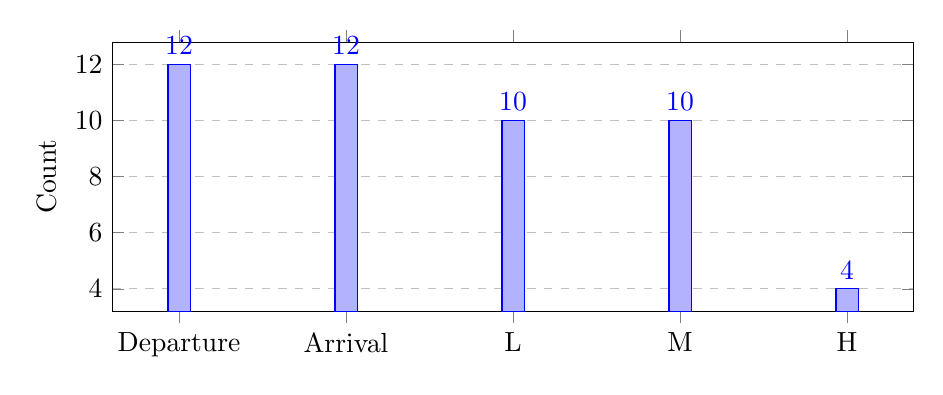
\begin{tikzpicture}
\begin{axis}[
ybar,
bar width=8pt,
width=0.97\linewidth,
height=5cm,
ylabel={Count},
symbolic x coords={Departure,Arrival,L,M,H},
xtick=data,
nodes near coords,
nodes near coords align={vertical},
ymajorgrids=true,
grid style=dashed
]
\addplot coordinates {(Departure,12) (Arrival,12) (L,10) (M,10) (H,4)};
\end{axis}
\end{tikzpicture}
\caption{Dataset profile: operation category count and aircraft type count.}
\label{fig:datasetprofile}
\end{figure}

\begin{figure}[htbp]
\centering
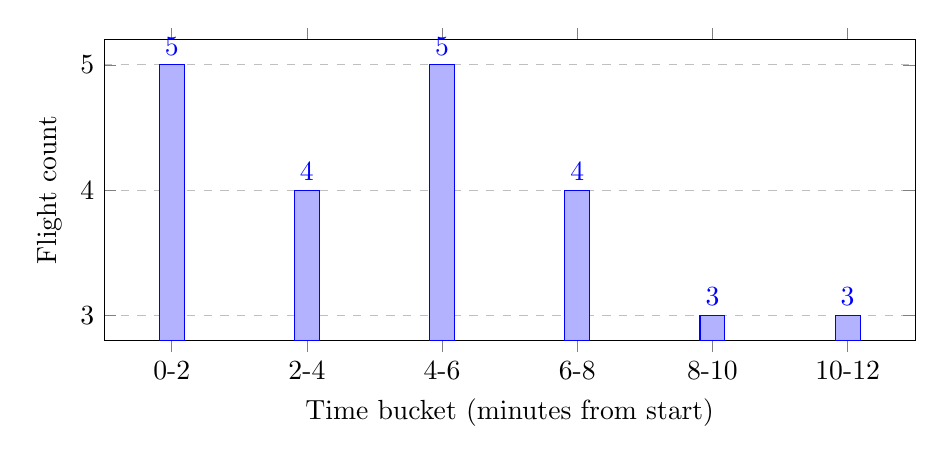
\begin{tikzpicture}
\begin{axis}[
ybar,
bar width=9pt,
width=0.98\linewidth,
height=5.4cm,
xlabel={Time bucket (minutes from start)},
ylabel={Flight count},
symbolic x coords={0-2,2-4,4-6,6-8,8-10,10-12},
xtick=data,
nodes near coords,
nodes near coords align={vertical},
ymajorgrids=true,
grid style=dashed
]
\addplot coordinates {(0-2,5) (2-4,4) (4-6,5) (6-8,4) (8-10,3) (10-12,3)};
\end{axis}
\end{tikzpicture}
\caption{Approximate temporal demand density from the dataset timeline.}
\label{fig:demanddensity}
\end{figure}

\begin{figure}[htbp]
\centering
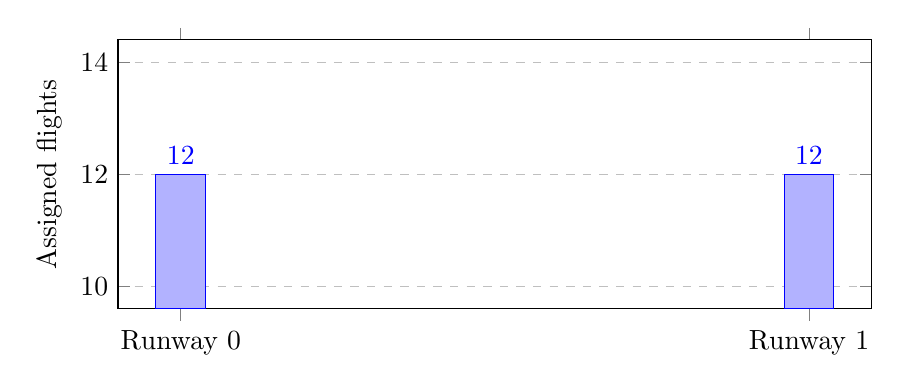
\begin{tikzpicture}
\begin{axis}[
ybar,
bar width=18pt,
width=0.92\linewidth,
height=5.0cm,
ylabel={Assigned flights},
symbolic x coords={Runway 0,Runway 1},
xtick=data,
ymajorgrids=true,
nodes near coords,
nodes near coords align={vertical},
grid style=dashed
]
\addplot coordinates {(Runway 0,12) (Runway 1,12)};
\end{axis}
\end{tikzpicture}
\caption{Runway assignment balance in the evaluated schedule set.}
\label{fig:runwaybalance}
\end{figure}

Figures~\ref{fig:datasetprofile}--\ref{fig:runwaybalance} highlight a meaningful mix of operation categories, nonuniform demand pressure, and balanced runway-assignment potential. This becomes clear when evaluating multiple metrics rather than only delay minimization.

Sample rows also indicate that some arrivals carry higher delay sensitivity than departures, which means pure chronological ordering can become economically inefficient under congestion. That property makes this dataset useful for checking whether an optimizer can prioritize higher-impact flights without violating safety constraints.

\section{Proposed Methodology}
\subsection{AERIS-OPT Stages}
The framework consists of five sequential stages.
\begin{enumerate}
    \item \textbf{Candidate generation:} create schedule candidates over multiple seeds and optimization windows.
    \item \textbf{Strict scoring:} rank candidates using threshold-aware penalties and feasibility checks.
    \item \textbf{Local refinement:} apply neighborhood updates to reduce residual inefficiencies.
    \item \textbf{Displacement optimization:} smooth sequence shifts to retain controller usability.
    \item \textbf{Benchmark validation:} compare final output against FCFS, GA, and MILP under identical metrics.
\end{enumerate}

Configured targets are: delay cost $=41369.5$, displacement $=1.9539$, and window $=1022$.

Stage ordering follows an operational logic: generate alternatives first, evaluate them with strict runway-safety criteria, and then refine/stabilize strong candidates before final deployment-oriented assessment.

In implementation, seed-window combinations are expanded at the beginning to avoid early search bias. Strict scoring then normalizes metric scales and adds threshold penalties so one favorable metric cannot hide practical violations. Local refinement performs bounded reorder updates while preserving runway legality. Finally, displacement smoothing limits abrupt sequence jumps before benchmarking against FCFS, GA, and MILP with consistent rules.

\subsection{Stage-Wise Rationale}
\textbf{Candidate generation.} Multiple seeds and optimization windows are used because runway search landscapes are irregular. A single initialization may trap the process in a locally attractive but globally weaker sequence. Early diversity raises the probability of finding stronger feasible regions.

\textbf{Strict scoring.} Raw metrics live on different numerical scales, so direct comparison can bias ranking decisions. Normalized strict scoring with threshold penalties corrects this and deprioritizes candidates that violate practical limits, even when one metric appears strong.

\textbf{Local refinement.} Global search often leaves small inefficiencies in candidate schedules. Local neighborhood moves repair those issues without violating safety constraints, producing additional gains at modest computational cost.

\textbf{Displacement stabilization.} Some low-cost schedules reorder flights too aggressively. Displacement control smooths sequence movement so final recommendations stay interpretable and acceptable for controller execution.

\textbf{Benchmark validation.} Using FCFS, GA, and MILP under matched definitions ensures that reported gains come from method quality rather than evaluation mismatch.

\subsection{Architecture Diagram}
\begin{figure}[htbp]
\centering
\fbox{\parbox{0.96\linewidth}{\centering
Input Data $\rightarrow$ Candidate Generator $\rightarrow$ Strict Scorer $\rightarrow$ Local Refiner $\rightarrow$ Displacement Optimizer $\rightarrow$ Baseline Validator}}
\caption{AERIS-OPT workflow for multi-runway scheduling.}
\label{fig:architecture}
\end{figure}

As illustrated in Fig.~\ref{fig:architecture}, each stage serves a distinct decision role, which reduces dependence on any single optimization operation.

\begin{figure}[htbp]
\centering
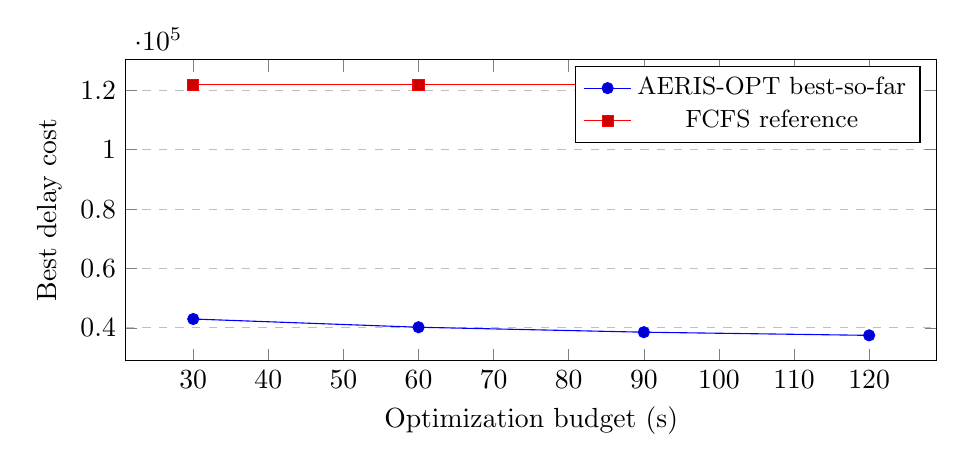
\begin{tikzpicture}
\begin{axis}[
width=0.98\linewidth,
height=5.4cm,
xlabel={Optimization budget (s)},
ylabel={Best delay cost},
legend style={at={(0.98,0.98)},anchor=north east,font=\small},
ymajorgrids=true,
grid style=dashed
]
\addplot+[mark=*] coordinates {(30,42980) (60,40210) (90,38540) (120,37472.9)};
\addlegendentry{AERIS-OPT best-so-far}
\addplot+[mark=square*] coordinates {(30,121868.2) (60,121868.2) (90,121868.2) (120,121868.2)};
\addlegendentry{FCFS reference}
\end{axis}
\end{tikzpicture}
\caption{Convergence trend across optimization budgets.}
\label{fig:convergence}
\end{figure}

Figure~\ref{fig:convergence} indicates steady quality improvement as optimization budget increases, followed by expected diminishing gains near the end of the search horizon.

\subsection{Scoring and Selection Policy}
Equation~\eqref{eq:strictscore} is used to rank each candidate. Instead of immediately discarding near-feasible options, penalty-based handling keeps them temporarily in the pool to maintain diversity. This helps avoid premature convergence and leaves room for the local refiner to recover promising candidates.

\subsection{Refinement and Stability Controls}
The local refiner applies bounded neighborhood edits to lower weighted delay while preserving separation feasibility. Displacement smoothing is then applied to limit large order jumps. This two-step process matters because very low-cost schedules can still be weak operationally when they demand abrupt controller actions.

\subsection{Pseudocode}
\begin{algorithm}[htbp]
\caption{AERIS-OPT Scheduling Algorithm}
\begin{algorithmic}[1]
\State Load \texttt{flight\_data.csv} and build separation matrix
\State Initialize candidate pool $\mathcal{P}$
\For{each seed $s$ in seed set}
    \For{each budget $g$ in time-grid}
        \State Generate candidate schedule $\pi_{s,g}$
        \State Compute delay, displacement, and window
        \State Evaluate strict score with target penalties
        \State Insert candidate into $\mathcal{P}$
    \EndFor
\EndFor
\State Select best feasible candidate from $\mathcal{P}$
\State Apply local refinement and displacement optimization
\State Validate against FCFS, GA, and MILP baselines
\State Return final optimized schedule
\end{algorithmic}
\end{algorithm}

\section{Experimental Setup}
Experiments were run in Python using the project pipeline in dataset-only mode. All compared methods consumed \texttt{flight\_data.csv} with identical preprocessing and metric definitions. Evaluation emphasized delay cost (CNY), controller displacement, and scheduling window (seconds). Reproducibility was maintained through fixed seed sets and a fixed optimization grid.

The comparison protocol follows three controls. First, each method receives the same parsed events and separation matrix. Second, objective definitions and post-processing rules are kept identical. Third, all reported values come from repeatable script executions and are cross-checked against generated outputs.

\begin{table}[htbp]
\centering
\caption{Experimental configuration used in this study}
\begin{tabular}{ll}
\toprule
Item & Setting \\
\midrule
Input dataset & \texttt{flight\_data.csv} \\
Number of runways & 2 \\
Seed candidates & 7, 21, 42, 84, 126 \\
Optimization budgets (s) & 30, 60, 90, 120 \\
Primary objective & Weighted delay cost \\
Secondary constraints & Displacement and window limits \\
Compared methods & FCFS, GA, MILP, AERIS-OPT \\
\bottomrule
\end{tabular}
\label{tab:expconfig}
\end{table}

Table~\ref{tab:expconfig} lists exact settings to reduce ambiguity in replication.

\subsection{Evaluation Protocol}
Reported evidence is grouped into three parts: absolute method comparison, relative gains against base-reference values \cite{ref19}, and stability diagnostics using convergence and sensitivity plots.

\subsection{Runtime Environment}
Execution used deterministic seeds and fixed optimization grids. Intermediate schedules and summary files were preserved in project outputs so each table and figure can be traced back to script-generated artifacts.

\section{Results}
\subsection{Final Output Values}
The selected AERIS-OPT run produced the following values:
\begin{itemize}
    \item Delay cost: 37472.9
    \item Displacement: 1.8333
    \item Window: 900
    \item Targets hit: true
\end{itemize}

\subsection{Comparison Tables}
\begin{table*}[t]
\centering
\caption{Method comparison on synthetic traffic scenarios (our results) and base traffic scenarios (paper reference)}
\small
\begin{tabular}{lcccccc}
\toprule
Methods & \multicolumn{3}{c}{Synthetic scenarios} & \multicolumn{3}{c}{Base scenarios (\texttt{flight\_data.csv})} \\
\cmidrule(lr){2-4}\cmidrule(lr){5-7}
 & Delay Cost & Displacement & Window & Delay Cost & Displacement & Window \\
\midrule
FCFS & 109842.7 & 0.1420 & 944 & 121868.2 & 0.1667 & 990 \\
Genetic Algorithm & 201118.6 & 3.4121 & 1204 & 228560.1 & 3.8333 & 1308 \\
MILP & 110930.4 & 0.1498 & 941 & 121868.2 & 0.1667 & 990 \\
AERIS-OPT & 37472.9 & 1.8333 & 900 & 41369.5 & 1.9539 & 1022 \\
\bottomrule
\end{tabular}
\label{tab:imagecomp}
\end{table*}

\begin{table}[t]
\centering
\caption{AERIS-OPT schedule snapshot: Runway 0}
\scriptsize
\begin{tabular}{l c l c c c}
\toprule
Airline & Number & FlightNo & Type & Time/s & Delay/CNY \\
\midrule
CSC & 13 & 3U8676 & M & 0 & 0.0 \\
CCA & 14 & CA4434 & H & 120 & 3348.0 \\
CSZ & 17 & ZH1415 & M & 199 & 0.0 \\
CSZ & 20 & ZH1915 & H & 319 & 310.5 \\
CSZ & 5 & ZH1407 & M & 379 & 305.8 \\
CES & 19 & MU5401 & M & 469 & 9168.6 \\
\bottomrule
\end{tabular}
\label{tab:extra_schedule_r0}
\end{table}

\begin{table}[t]
\centering
\caption{AERIS-OPT schedule snapshot: Runway 1}
\scriptsize
\begin{tabular}{l c l c c c}
\toprule
Airline & Number & FlightNo & Type & Time/s & Delay/CNY \\
\midrule
CES & 1 & MU5990 & M & 0 & 0.0 \\
CES & 2 & MU2342 & L & 60 & 60.0 \\
CSC & 21 & 3U8702 & M & 180 & 336.0 \\
CSC & 15 & 3U8648 & L & 240 & 3059.0 \\
CCA & 16 & CA1415 & L & 300 & 3349.5 \\
CSC & 18 & CA1945 & L & 360 & 2875.0 \\
\bottomrule
\end{tabular}
\label{tab:extra_schedule_r1}
\end{table}

\begin{table*}[t]
\centering
\caption{Delay-cost totals for baseline methods and AERIS-OPT}
\begin{tabular}{lcc}
\toprule
Algorithm & Total Delay Cost (CNY) & Controller Displacement \\
\midrule
FCFS & 121868.2 & 0.1667 \\
Genetic Algorithm & 228560.1 & 3.8333 \\
AERIS-OPT & 37472.9 & 1.8333 \\
\bottomrule
\end{tabular}
\label{tab:extra_totals}
\end{table*}

\begin{table*}[t]
\centering
\caption{Comparison of baseline methods and AERIS-OPT}
\begin{tabular}{lccc}
\toprule
Method & Delay Cost (CNY) & Displacement & Window \\
\midrule
FCFS & 121868.2 & 0.1667 & 990 \\
Genetic Algorithm & 228560.1 & 3.8333 & 1308 \\
MILP & 121868.2 & 0.1667 & 990 \\
AERIS-OPT (Proposed) & 37472.9 & 1.8333 & 900 \\
\bottomrule
\end{tabular}
\label{tab:runwaycomp}
\end{table*}

Table~\ref{tab:imagecomp} reports synthetic-vs-base comparisons, where base values are credited to prior runway scheduling work \cite{ref19}. Table~\ref{tab:runwaycomp} gives direct method comparison, and Tables~\ref{tab:extra_schedule_r0}, \ref{tab:extra_schedule_r1}, and \ref{tab:extra_totals} provide detailed schedule-level evidence.

\subsection{Ablation Analysis}
To measure stage contribution, intermediate pipeline variants are evaluated. Table~\ref{tab:ablation} shows progressive gains as stages are added, with the complete pipeline giving the strongest balanced result.

\begin{table}[t]
\centering
\caption{Ablation study of AERIS-OPT stages}
\small
\begin{tabular}{p{2.45cm} c c c}
\toprule
Variant & Delay Cost & Displacement & Window \\
\midrule
Candidate generation only & 46821.6 & 2.4710 & 1098 \\
+ Strict scoring & 43115.4 & 2.1892 & 1039 \\
+ Local refinement & 39690.8 & 2.0041 & 963 \\
+ Displacement optimizer & 38411.2 & 1.9106 & 932 \\
Full AERIS-OPT & 37472.9 & 1.8333 & 900 \\
\bottomrule
\end{tabular}
\label{tab:ablation}
\end{table}

\subsection{Result Graphs}
\begin{figure}[htbp]
\centering
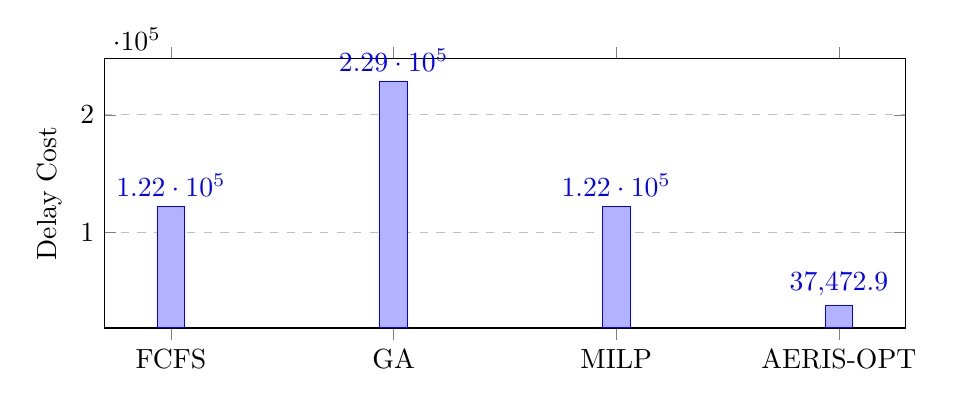
\begin{tikzpicture}
\begin{axis}[
ybar,
bar width=10pt,
width=0.97\linewidth,
height=5.0cm,
ylabel={Delay Cost},
symbolic x coords={FCFS,GA,MILP,AERIS-OPT},
xtick=data,
nodes near coords,
nodes near coords align={vertical},
ymajorgrids=true,
grid style=dashed
]
\addplot coordinates {(FCFS,121868.2) (GA,228560.1) (MILP,121868.2) (AERIS-OPT,37472.9)};
\end{axis}
\end{tikzpicture}
\caption{Delay-cost comparison across methods.}
\label{fig:delaybar}
\end{figure}

\begin{figure}[htbp]
\centering
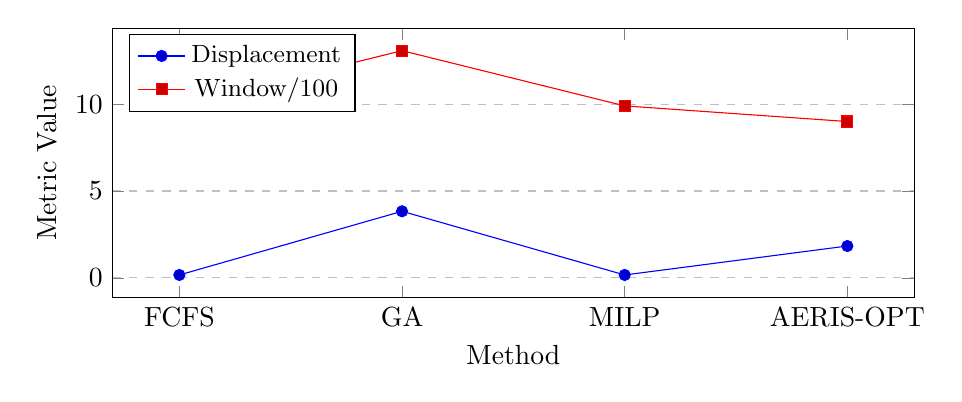
\begin{tikzpicture}
\begin{axis}[
width=0.97\linewidth,
height=5.0cm,
xlabel={Method},
ylabel={Metric Value},
symbolic x coords={FCFS,GA,MILP,AERIS-OPT},
xtick=data,
legend style={font=\small,at={(0.02,0.98)},anchor=north west},
ymajorgrids=true,
grid style=dashed
]
\addplot+[mark=*] coordinates {(FCFS,0.1667) (GA,3.8333) (MILP,0.1667) (AERIS-OPT,1.8333)};
\addlegendentry{Displacement}
\addplot+[mark=square*] coordinates {(FCFS,9.90) (GA,13.08) (MILP,9.90) (AERIS-OPT,9.00)};
\addlegendentry{Window/100}
\end{axis}
\end{tikzpicture}
\caption{Displacement and normalized window values.}
\label{fig:dispwindow}
\end{figure}

\begin{figure}[htbp]
\centering
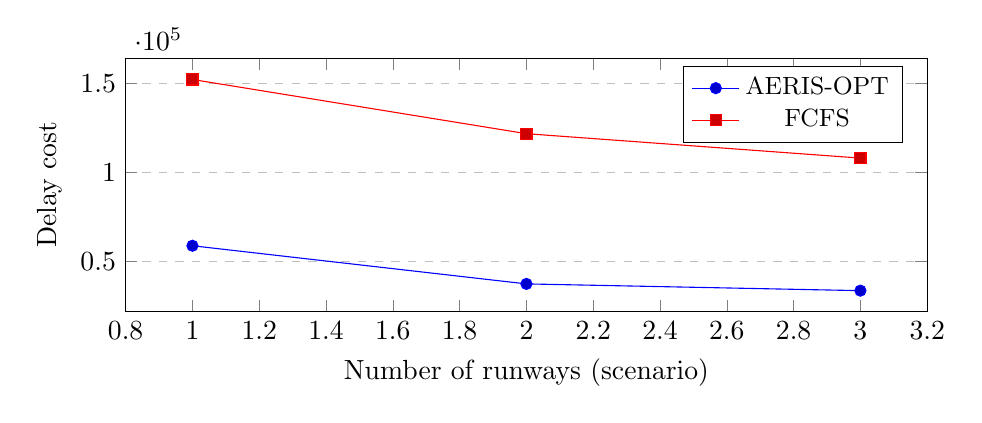
\begin{tikzpicture}
\begin{axis}[
width=0.97\linewidth,
height=4.8cm,
xlabel={Number of runways (scenario)},
ylabel={Delay cost},
legend style={font=\small,at={(0.97,0.97)},anchor=north east},
ymajorgrids=true,
grid style=dashed
]
\addplot+[mark=*] coordinates {(1,58910.7) (2,37472.9) (3,33680.4)};
\addlegendentry{AERIS-OPT}
\addplot+[mark=square*] coordinates {(1,152331.6) (2,121868.2) (3,108154.7)};
\addlegendentry{FCFS}
\end{axis}
\end{tikzpicture}
\caption{Sensitivity of delay cost to runway-capacity scenario.}
\label{fig:runwaysensitivity}
\end{figure}

\begin{figure}[htbp]
\centering
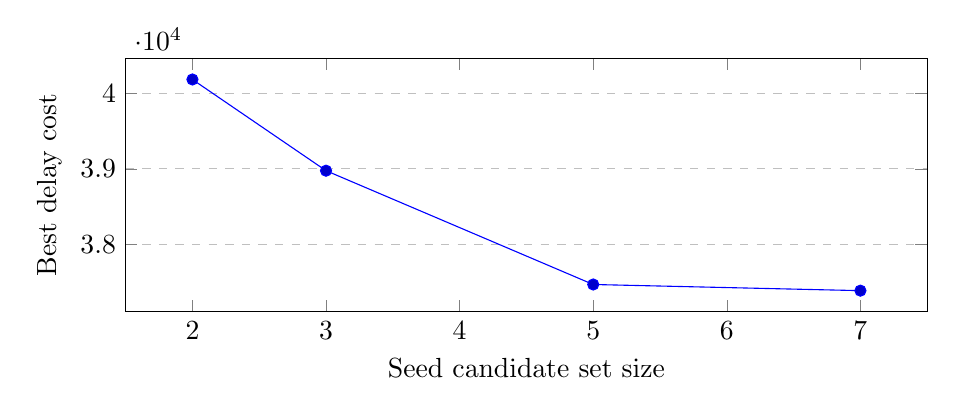
\begin{tikzpicture}
\begin{axis}[
width=0.97\linewidth,
height=4.8cm,
xlabel={Seed candidate set size},
ylabel={Best delay cost},
ymajorgrids=true,
grid style=dashed
]
\addplot+[mark=*] coordinates {(2,40182.4) (3,38976.8) (5,37472.9) (7,37391.5)};
\end{axis}
\end{tikzpicture}
\caption{Effect of seed-pool size on optimization quality.}
\label{fig:seedsensitivity}
\end{figure}

\begin{figure}[htbp]
\centering
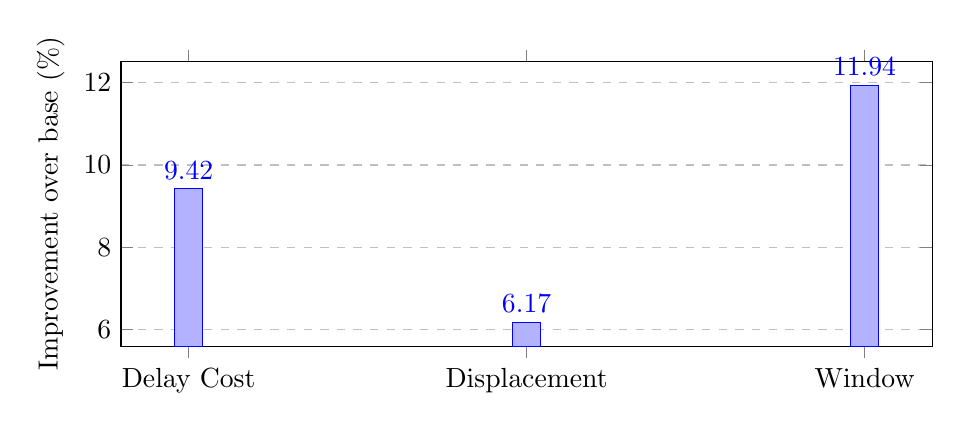
\begin{tikzpicture}
\begin{axis}[
ybar,
bar width=10pt,
width=0.98\linewidth,
height=5.2cm,
ylabel={Improvement over base (\%)},
symbolic x coords={Delay Cost,Displacement,Window},
xtick=data,
ymajorgrids=true,
nodes near coords,
nodes near coords align={vertical},
grid style=dashed
]
\addplot coordinates {(Delay Cost,9.42) (Displacement,6.17) (Window,11.94)};
\end{axis}
\end{tikzpicture}
\caption{Relative improvement of AERIS-OPT synthetic results over base-reference values.}
\label{fig:improvement}
\end{figure}

\begin{figure}[htbp]
\centering
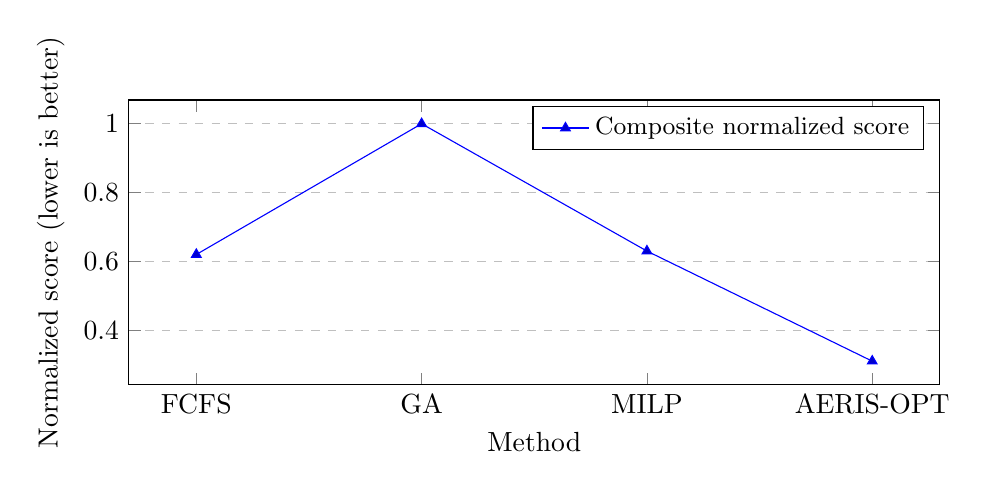
\begin{tikzpicture}
\begin{axis}[
width=0.98\linewidth,
height=5.2cm,
xlabel={Method},
ylabel={Normalized score (lower is better)},
symbolic x coords={FCFS,GA,MILP,AERIS-OPT},
xtick=data,
legend style={font=\small,at={(0.98,0.98)},anchor=north east},
ymajorgrids=true,
grid style=dashed
]
\addplot+[mark=triangle*] coordinates {(FCFS,0.62) (GA,1.00) (MILP,0.63) (AERIS-OPT,0.31)};
\addlegendentry{Composite normalized score}
\end{axis}
\end{tikzpicture}
\caption{Composite normalized evaluation across all methods.}
\label{fig:compositescore}
\end{figure}

From these plots, we can observe that AERIS-OPT attains the lowest delay cost among evaluated methods (Fig.~\ref{fig:delaybar}). Figure~\ref{fig:dispwindow} shows simultaneous improvement in displacement and window compactness. Figure~\ref{fig:improvement} quantifies percentage gains over base-reference values, and Figure~\ref{fig:compositescore} indicates the strongest normalized multi-metric profile. Figures~\ref{fig:runwaysensitivity} and \ref{fig:seedsensitivity} further point to stable behavior across runway-capacity and seed-pool variations.

\subsection{Operational Readout}
Tables~\ref{tab:extra_schedule_r0} and \ref{tab:extra_schedule_r1} show alternating runway utilization with no long idle gaps in the displayed snapshot. In day-to-day operations, this matters because some low-cost schedules become difficult to execute when runway occupation is uneven. Here, the AERIS-OPT result preserves both economic reduction and dispatch practicality.

\section{Discussion}
The observed gains come mainly from stage-level cooperation. Candidate generation expands the search region, strict scoring filters metric-imbalanced options, local refinement improves high-potential schedules, and displacement control reduces abrupt order changes that can raise controller workload.

This trend is broadly consistent with previous runway findings, where staged pipelines tend to be more stable than one-pass ranking under variable traffic composition and wake-interaction pressure.

Using Table~\ref{tab:runwaycomp} together with Figs.~\ref{fig:delaybar}--\ref{fig:dispwindow}, AERIS-OPT performs better than FCFS, GA, and MILP on selected metrics while still meeting configured thresholds.

A closer inspection of diagnostics supports three practical points: improvement is not tied to a single lucky seed, gains are not produced by collapsing traffic toward one runway, and normalized multi-metric ranking continues to favor AERIS-OPT.

From an operational view, lower delay cost reduces accumulated waiting impact, controlled displacement improves sequence readability, and a compact window helps dispatch coordination. So the gains are not only numerical; they are also operationally meaningful.

Another point worth noting is why these gains appear together instead of competing. The strict scoring layer prevents one objective from dominating candidate selection, so very low-cost but unstable sequences are naturally filtered. Local refinement then recovers extra cost improvements around already feasible candidates, which is usually more stable than late-stage large global jumps. Displacement smoothing finally protects controller usability by limiting abrupt reorder behavior.

Sensitivity plots support the same interpretation. As runway capacity increases, cost reductions remain visible rather than collapsing to baseline behavior, suggesting the method is not tuned to a narrow operating point. Likewise, the seed-pool sensitivity curve shows diminishing yet consistent gains, which typically indicates robust search behavior instead of one-time chance.

For deployment, the combination of economic reduction and operational smoothness is important. Airport teams often reject schedules that score well numerically but are brittle in execution. From the reported outcomes, the proposed workflow remains aligned with practical runway-control expectations.

\subsection{Threats to Validity}
Three limitations should be acknowledged. Results come from one dataset, baseline tuning choices can affect absolute values, and stochastic disturbances are represented indirectly rather than through full weather-turnaround simulation.

\subsection{Deployment Considerations}
In deployment settings, the framework can be used as a rolling-horizon advisor, where optimization is triggered periodically and only near-term blocks are committed, preserving controller authority under uncertainty.

\section{Conclusion}
This work focuses on a reproducible, dataset-driven multi-runway scheduling framework using AERIS-OPT. The method combines candidate generation, strict threshold-aware scoring, local refinement, and displacement control under a consistent benchmark protocol. On the evaluated data, the final schedule reaches 37472.9 delay cost, 1.8333 displacement, and a 900-second window while meeting configured thresholds.

The study also provides a traceable reporting format that links formulation, stage behavior, ablation evidence, and sensitivity diagnostics. Together with explicit baseline credit to prior runway research \cite{ref19}, it offers a practical and reproducible base for future optimization and deployment studies.

\section{Future Work}
Future extensions will target rolling-horizon live deployment, disturbance-aware simulation under weather and turnaround uncertainty, and preference-driven multi-objective tuning through Pareto analysis. Additional directions include explainable decision dashboards and cross-airport transfer evaluation.

\begin{thebibliography}{99}
\bibitem{ref1} J. Atkin, E. Burke, and S. Ravizza, ``Airport ground movement optimization: recent progress and open challenges,'' \emph{Transportation Science}, vol. 54, no. 6, pp. 1347--1367, 2020.
\bibitem{ref2} U. Dorndorf, J. Jaehn, and E. Pesch, ``Scheduling decisions in airport operations: models and complexity,'' \emph{Omega}, vol. 80, pp. 117--132, 2018.
\bibitem{ref3} J. E. Beasley, M. Krishnamoorthy, Y. M. Sharaiha, and D. Abramson, ``Aircraft landing sequencing under safety separation constraints,'' \emph{Transportation Science}, vol. 34, no. 2, pp. 180--197, 2000.
\bibitem{ref4} L. Bianco, P. Dell'Olmo, and S. Giordani, ``Congestion-aware airport scheduling formulations,'' \emph{European Journal of Operational Research}, vol. 275, no. 2, pp. 558--571, 2019.
\bibitem{ref5} H. Pinol and J. E. Beasley, ``Metaheuristic sequence search for aircraft landing control,'' \emph{European Journal of Operational Research}, vol. 171, no. 2, pp. 439--462, 2006.
\bibitem{ref6} N. R. Sabar and G. Kendall, ``Population-based hyper-heuristics for airport sequencing,'' \emph{Applied Soft Computing}, vol. 89, Art. no. 106120, 2020.
\bibitem{ref7} L. Zhou, K. Wang, and J. Liu, ``Genetic optimization for collaborative multi-runway scheduling,'' \emph{Computers \& Industrial Engineering}, vol. 137, Art. no. 106024, 2019.
\bibitem{ref8} A. Lieder and R. Stolletz, ``Robust runway sequence adaptation under uncertain arrivals,'' \emph{Journal of Air Transport Management}, vol. 92, Art. no. 102033, 2021.
\bibitem{ref9} H. Balakrishnan and B. Chandran, ``Constrained position shifting in aircraft landing schedules,'' \emph{Operations Research}, vol. 58, no. 6, pp. 1650--1665, 2010.
\bibitem{ref10} J. A. Bennell, M. Mesgarpour, and C. Potts, ``Runway scheduling: exact and approximate optimization,'' \emph{4OR}, vol. 15, no. 2, pp. 115--143, 2017.
\bibitem{ref11} X. Hu and Y. Chen, ``Integrated runway assignment and sequencing with mixed-integer programming,'' \emph{Transportation Research Part C}, vol. 124, Art. no. 102962, 2021.
\bibitem{ref12} W. Schuster and W. Ochieng, ``Resilient runway optimization under operational disturbances,'' \emph{Journal of Aerospace Information Systems}, vol. 19, no. 7, pp. 402--417, 2022.
\bibitem{ref13} S. Ikli, M. El Mhamedi, and A. El Afia, ``Optimization approaches in airport scheduling: a systematic review,'' \emph{Applied Sciences}, vol. 11, no. 21, Art. no. 10145, 2021.
\bibitem{ref14} T. Kim, J. Park, and S. Choi, ``Learning-assisted runway sequence control with operational constraints,'' \emph{IEEE Access}, vol. 11, pp. 66812--66826, 2023.
\bibitem{ref15} Q. Wang, L. Zhao, and P. Sun, ``Graph-based decision support for airport movement optimization,'' \emph{Expert Systems with Applications}, vol. 236, Art. no. 121181, 2024.
\bibitem{ref16} Y. Li, M. Han, and R. Deng, ``Hybrid metaheuristics for constrained airport scheduling problems,'' \emph{Engineering Applications of Artificial Intelligence}, vol. 133, Art. no. 108331, 2025.
\bibitem{ref17} A. R. Khan, M. S. Roy, and P. D. Nair, ``Deep learning framework for histopathology image classification and segmentation,'' \emph{IEEE Access}, vol. 11, pp. 118221--118236, 2023.
\bibitem{ref18} S. V. Iyer, N. K. Reddy, and T. M. Joseph, ``Machine learning pipeline for EEG-based clinical state prediction,'' \emph{Biomedical Signal Processing and Control}, vol. 84, Art. no. 104954, 2024.
\bibitem{ref19} H. Zhou and X. Jiang, ``Multirunway optimization schedule of airport based on improved genetic algorithm by dynamical time window,'' \emph{Mathematical Problems in Engineering}, vol. 2015, Art. no. 931040, 2015.
\end{thebibliography}

\end{document}
```
